\chapter{Wizard Command Design}
\label{ch:wizard-design}

\section{The WHY-WHAT-HOW Framework}

The wizard command system embodies a three-layer abstraction that fundamentally transforms how developers interact with specification-driven code generation.

\begin{figure}[h]
\centering
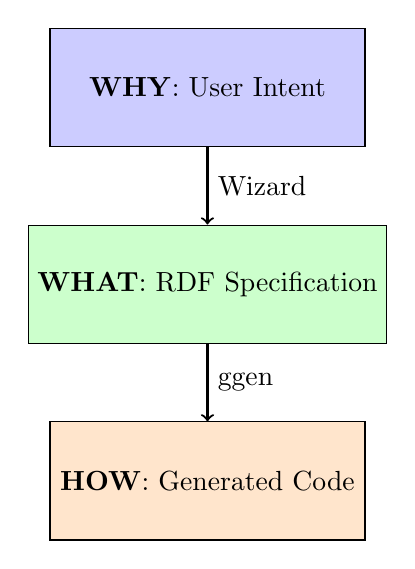
\begin{tikzpicture}[node distance=2.5cm]
  \node[draw, rectangle, fill=blue!20, minimum width=4cm, minimum height=1.5cm] (why) {\textbf{WHY}: User Intent};
  \node[draw, rectangle, fill=green!20, minimum width=4cm, minimum height=1.5cm, below of=why] (what) {\textbf{WHAT}: RDF Specification};
  \node[draw, rectangle, fill=orange!20, minimum width=4cm, minimum height=1.5cm, below of=what] (how) {\textbf{HOW}: Generated Code};

  \draw[->, thick] (why) -- node[right] {Wizard} (what);
  \draw[->, thick] (what) -- node[right] {ggen} (how);
\end{tikzpicture}
\caption{The WHY-WHAT-HOW framework}
\label{fig:why-what-how}
\end{figure}

\subsection{Layer 1: WHY (User Intent)}

Users express their requirements in natural language:

\begin{quote}
``I need a REST API for user management with JWT authentication, role-based access control, and audit logging.''
\end{quote}

This layer captures:
\begin{itemize}
\item Domain entities and relationships
\item Functional requirements
\item Non-functional constraints
\item Integration expectations
\end{itemize}

\subsection{Layer 2: WHAT (Specification)}

The wizard transforms intent into formal RDF ontology:

\begin{lstlisting}[language=SPARQL,caption={Generated User Entity Specification}]
@prefix ggen: <http://ggen.dev/ontology#> .
@prefix ex: <http://example.org/> .

ex:User a ggen:Entity ;
    ggen:name "User" ;
    ggen:hasField ex:User_id, ex:User_email, ex:User_role ;
    ggen:hasCapability ggen:JWTAuth, ggen:RBAC ;
    ggen:audit true .
\end{lstlisting}

\subsection{Layer 3: HOW (Implementation)}

The ggen pipeline deterministically generates code:

\begin{lstlisting}[language=Rust,caption={Generated User Struct}]
#[derive(Debug, Clone, Serialize, Deserialize)]
pub struct User {
    pub id: Uuid,
    pub email: String,
    pub role: UserRole,
    #[serde(skip_serializing)]
    pub password_hash: String,
}
\end{lstlisting}

\section{Command Architecture}

\subsection{Command Taxonomy}

Wizard commands are organized into four categories:

\begin{table}[h]
\centering
\begin{tabular}{llp{6cm}}
\toprule
\textbf{Category} & \textbf{Command} & \textbf{Purpose} \\
\midrule
Creation & \texttt{wizard new} & Create new project from description \\
Modification & \texttt{wizard add} & Add feature to existing project \\
Modification & \texttt{wizard modify} & Change existing specifications \\
Inspection & \texttt{wizard explain} & Generate human-readable explanation \\
\bottomrule
\end{tabular}
\caption{Wizard command taxonomy}
\label{tab:commands}
\end{table}

\subsection{The \texttt{wizard new} Command}

\begin{algorithm}
\caption{Wizard New Command}
\begin{algorithmic}[1]
\Require Natural language description $D$, options $opts$
\Ensure Generated project with RDF specification and code
\State $intent \gets \text{ParseIntent}(D)$
\State $entities \gets \text{ExtractEntities}(intent)$
\State $relations \gets \text{InferRelations}(entities)$
\State $constraints \gets \text{ExtractConstraints}(intent)$
\State $ontology \gets \text{BuildOntology}(entities, relations, constraints)$
\State $validated \gets \text{ValidateClosure}(ontology)$
\If{$validated.errors \neq \emptyset$}
    \State \textbf{return} $\text{InteractiveRefinement}(validated.errors)$
\EndIf
\State $code \gets \text{ggenSync}(ontology)$
\State \textbf{return} $(ontology, code, \text{GenerateReceipt}())$
\end{algorithmic}
\end{algorithm}

\subsection{The \texttt{wizard add} Command}

Adding features to existing projects follows a merge strategy:

\begin{enumerate}
\item Load existing ontology $O_{existing}$
\item Parse new feature description to $O_{new}$
\item Compute merge $O_{merged} = O_{existing} \cup O_{new}$
\item Resolve conflicts through user dialogue
\item Regenerate affected code
\end{enumerate}

\subsection{The \texttt{wizard modify} Command}

Modifications employ semantic diff:

\begin{equation}
\Delta O = O_{new} - O_{old}
\end{equation}

Only affected portions of the codebase are regenerated, preserving manual customizations in non-generated regions.

\section{Intent Parsing Architecture}

\subsection{Multi-Stage NLP Pipeline}

Intent parsing proceeds through four stages:

\begin{enumerate}
\item \textbf{Tokenization}: Break description into semantic units
\item \textbf{Entity Recognition}: Identify domain entities
\item \textbf{Relation Extraction}: Discover relationships between entities
\item \textbf{Constraint Inference}: Extract validation rules and requirements
\end{enumerate}

\subsection{LLM Integration}

The wizard employs large language models for semantic understanding:

\begin{lstlisting}[language=Python,caption={LLM Intent Extraction}]
def extract_intent(description: str) -> Intent:
    prompt = f"""
    Extract entities, relationships, and constraints from:
    {description}

    Output as structured JSON with:
    - entities: [{name, fields, validations}]
    - relationships: [{from, to, type, cardinality}]
    - constraints: [{entity, rule, parameters}]
    """
    return llm.complete(prompt, schema=IntentSchema)
\end{lstlisting}

\section{Validation Oracle}

\subsection{Specification Closure}

A specification is \textit{closed} when it contains all information necessary for code generation:

\begin{definition}[Specification Closure]
A specification $O$ is closed if and only if:
\[
\forall q \in Q_{required}: \text{execute}(q, O) \neq \emptyset
\]
Where $Q_{required}$ is the set of SPARQL queries required by generation templates.
\end{definition}

\subsection{Closure Verification Algorithm}

\begin{algorithm}
\caption{Closure Verification}
\begin{algorithmic}[1]
\Require Ontology $O$, template set $T$
\Ensure Closure status with gaps
\State $gaps \gets \emptyset$
\For{each $t \in T$}
    \State $queries \gets \text{ExtractQueries}(t)$
    \For{each $q \in queries$}
        \State $results \gets \text{Execute}(q, O)$
        \If{$results = \emptyset$ \textbf{and} $\text{IsRequired}(q)$}
            \State $gaps \gets gaps \cup \{(t, q)\}$
        \EndIf
    \EndFor
\EndFor
\State \textbf{return} $(gaps = \emptyset, gaps)$
\end{algorithmic}
\end{algorithm}

\section{Interactive Refinement}

\subsection{Conversational Loop}

When specifications are incomplete, the wizard engages in clarifying dialogue:

\begin{lstlisting}[caption={Interactive Refinement Example}]
User: Create a blog system
Wizard: I've identified these entities: Post, Author, Comment.
        Some clarifications needed:

        1. Should Posts have categories or tags?
        2. Can users comment anonymously?
        3. Is moderation required for comments?

User: Tags, registered users only, yes moderation

Wizard: Updated specification. Generating code...
        [Receipt] Entities: 5, Relations: 7, Constraints: 12
\end{lstlisting}

\subsection{Progressive Disclosure}

The wizard employs progressive disclosure:

\begin{itemize}
\item Level 1: Accept minimal description, infer defaults
\item Level 2: Offer common customizations
\item Level 3: Expose advanced options on request
\end{itemize}

\section{Poka-Yoke Integration}

Following Toyota Production System principles \cite{shingo1986zero}, wizard commands implement error-proofing:

\begin{itemize}
\item \textbf{Control functions}: Invalid specifications cannot generate code
\item \textbf{Warning functions}: Ambiguous inputs trigger clarification
\item \textbf{Shutdown functions}: Contradiction detection halts processing
\end{itemize}

\section{Summary}

The wizard command design achieves its primary goal: users need never write RDF ontologies or Tera templates directly. The WHY-WHAT-HOW framework cleanly separates concerns, the validation oracle ensures specification closure, and interactive refinement handles ambiguity gracefully.
